\chapter{Background}
\epigraph{
The genetic code does not, and cannot, specify the nature and position of every
capillary in the body or every neuron in the brain. What it can do is describe
the underlying fractal pattern which creates them.}{Academician Prokhor
Zakharov \\\textit{Sid Meier's Alpha Centauri}}
Creating a cyborg is a massive cross disciplinary effort, and if a scope is not
clearly defined the background runs the risk of becoming equally massive.
The goal of the thesis is to create a hybrid neuro-digital system capable of
controlling a simple robot, and by extension to create a ``bridge'' between
neural and digital.
Each section in the background shares this bridge as a red thread, and
consequently topics that are not directly related to the thesis' goal are discarded.
The background is laid out as follows:
First \emph{Complex Systems} are introduced as a framework to discuss the computational
capabilities in a wide range of systems that exhibit system dynamics similar to
that of neurons.
Modeling neurons as a complex systems is a first step towards establishing a
common ``language'' between neural activity and digital logic.
%
Next, \emph{Material Computing} and \emph{Evolution In Materio}, EiM for short,
introduces computation done in unstructured matter through the process of
evolution. The goals of EiM are closely aligned to the goal of this thesis, as
both study massively parallel computation happening in physical matter shaped by
the process of evolution.
%
Next section, \emph{Neurons As Computers} introduces neurons with a strong focus
on their computational capabilities.
Building on the EiM section, this section motivates a necessary reduction of
scope, proposing a simplified model of the computing neuron and a medium of
communication between neuron and digital.
%
Finally, \emph{Reservoir Computing} is introduced, tying together the previous
sections by introducing the framework of reservoir computing in order to
establish a common ``language'' between neural cultures and digital.
%
\section{Complex Systems}
%
Before discussing complex systems it is necessary to provide a definition of
complexity and system.
In common parlance complexity one might describe a book as complex due to its
intertwined narrative, where small details later turn into large plot points.
A song can be described as complex because of how the different instruments play
together, providing a context to the lyrics and vice versa.
Giving an exact of what complexity is is awkward, but the common theme is
highly interconnected interaction.
In the first example this refers to how the narratives intertwine, where no
narrative makes sense outside of the context of the other narratives, while in
the second example it refers to how the differenent instruments can interplay,
giving meaning to each other in such a way that one instrument alone, or the
lyrics simply written down loses meaning and impact.
\par
%
A system is defined as a set of elements and the relations between them.
When a system changes over time it is a \emph{dynamical} system, a property that
is implicitly assumed for the rest of this thesis.
When there are no interaction the system can only be described by its
constituent elements, and these systems are not very interesting.
When systems have interaction this interaction can be either linear or
\emph{nonlinear}.
Linear systems are characterized by the independence of interaction.
In these systems the behavior of the system as a whole is driven by the
interaction of components, but each individual component behaves independantly
of the rest of the system.
When designing systems this is a desirable property because it enables a
\emph{top down} design process where each part of a machine can be designed
independently before being put together, as each part does not alter its
behavior when part of a larger system, allowing us to assemble large systems
that are \emph{complicated} while keeping complexity low.
When the interactions become nonlinear this property is lost, and these systems
become very hard to reason about and design.
As Strogatz puts it, ``Whenever pants of a system interfere, cooperate or
compete there are nonlinear interactions going on. ...if you listen to your two
favorite songs at the same time you won't get double the pleasure!''
\cite{strogatz_nonlinear_2014}
In \emph{complex systems} nonlinear interaction is what shapes the systems
behavior which becomes greater than the sum of parts.
%
\subsubsection{Feedback and Self Organization}
The nonlinearity of interactions in complex systems is often expressed as
\emph{feedback} which when positive can amplify small perturbations into
cascading effects that change the system entirely, or when negative act as
dampeners, givin the system some measure of stability.
An example of this is how bees harvest nectar which must be carefully dried, a
process that can be done on a large scale if all the nectar has the same water
content.
Because of this a hive will harvest from only one source at a time, which in
beekeeping terms is known as ``flow'' (with raspberry-flow being the most
important one).
With no centralized decisionmaker the bees are still able to quickly agree on a
new flow once the current flow dries up through local interactions.
When a worker bee finds a suitable source of nectar it will fly back to the hive
and perform a dance, informing other bees of the food source.
Other bees that see this dance will then seek out the food source, and if
successful they too will return to the hive to recruit new workers, however even
after a successful foraging they can still be recruited to a different source.
Often several food sources are found, and these sources ``compete'' against each
other, but typically the closest source wins because the faster trips cause
recruitment to happen quicker.
Through the amplification of local effects (one bee finding a food source) the
bees settle on one type of nectar, a \emph{global behavior} that has
\emph{emerged} in a \emph{bottom up} fashion, i.e without the need for
a centralized decisionmaker through the process of \emph{self organization}.
Through collective behavior bees can adapt to changes in their environment, in
fact a hive may even survive the death of their queen by moving a worker larvae
to a queen cell.
To highlight how much of the bees sophistication arise from collective behavior,
consider the fact that if a hive is moved even a meter, the forager bees will
not be able to find their way back home, clearly as an individual the bee is not
a great thinker!
\par
%
Just like a bee does not operate in a vacuum, the beehive is part of a larger
ecosystem.
Local interactions on the \emph{scale} of a single bee shapes the behavior at
the scale of the entire hive, which in turn interacts with the surrounding flora
at the scale of the eco-system.
In short, every layer that is peeled away, from the scale of the eco-system to
the scale of local flora down to the scale of a single bee reveals a new layer
of complexity.
Changing the scale of observation does not only reveal new complexities, it can
just as well reveal simplicity and order.
An example of this \emph{emergent simplicity} is the earth itself which behaves
as a simple celestial body in the solar system regardless of the complexities
found in smaller scales of observation.
%
\subsubsection{State Spaces and Attractors}
The space of possible states, or configurations a system can be in is known as a
\emph{state space}\footnote{For continuous systems the word phase space is more
  accurate, but it's not a useful dichotomy for this thesis.}
As an example, the state space of a rubiks cube can be defined as all possible
configurations a cube can be in.
This space includes the solved cube as well as any permutation reachable from
the solved cube when twisting it, but it does not include impossible rubiks
cubes such as a cube with ten red faces.
A single system may be defined by multiple state spaces depending on which parts
of the system is observed and at which scale.
The state space of the rubiks cube can be extended to include the current
rotation the cube has in space, or it can be observed at a finer scale where two
solved cubes occupy different states if the face of one cube has been slightly
rotated.
These states are known as \emph{macro states} and have been chosen specifically
by the observer as opposed to the \emph{micro state} which is the ground truth
of the system.
For physical systems the micro state is not only intractable, but impossible to
measure due to the uncertainity principle, and generally what happens at a
subatomic level is not very relevant when describing a rubiks cube.\par
%
As a dynamic system evolves over time it follows a trajectory through its state
space which depends on its initial conditions and outside perturbance.
Analogous to gravity wells in cosmology, certain points in the state space act
as \emph{attractors}, ``pulling in'' the states in its \emph{attractor basin}.
The simplest such attractor is the point attractor in which a system in the
point attractors basin will move towards a static state.
Cyclic attractors are a sequence of states that repeat themselves sequentially.
A system in a cyclic attractor can oscillate between two states, or it can
follow a longer path, known as cycle length before repeating itself.
For both cyclic and point attractors the amount of states a system goes through
before reaching the attractor (that is, the amount of states visited only once)
is known as the \emph{transient}.
The length of the transient is a property of one trajectory leading to the
attractor, but the average trajectory length is a property of the attractor
itself.
There is a third type of attractor which have have no cycles, known as
\emph{strange attractors}.
Systems in strange attractors exhibits \emph{chaotic} behavior, characterized by
its sensitivity to initial conditions and unpredictable, seemingly random
behavior.
Fig \ref{figStrange} shows one solution for a nonlinear differential equation known
as Lorenz attractor.
Two near-identical initial conditions in a this attractor will quickly diverge in
behavior, however both will create the ``butterfly'' pattern.
For a discrete system a strange attractor is impossible as any discrete system
can only represent a finite amount of states, however a cyclic attractor with a
cycle length near the total amount of expressible states may be informally
considered as strange.
% 
% TODO: Something about attractor landscape wrt complex, chaotic and ordered systems.
% A state space along with its attractor is known as an \emph{attractor
%   landscape}.
% Based on the attractor landscape the system can then be classified as ordered,
% complex or chaotic, however as examplified with the rubiks cube, the choice of
% macro state and observation scale means that these classifications are not
% objective as they also depend on the observer.
\begin{figure}[h!]
  \centering
  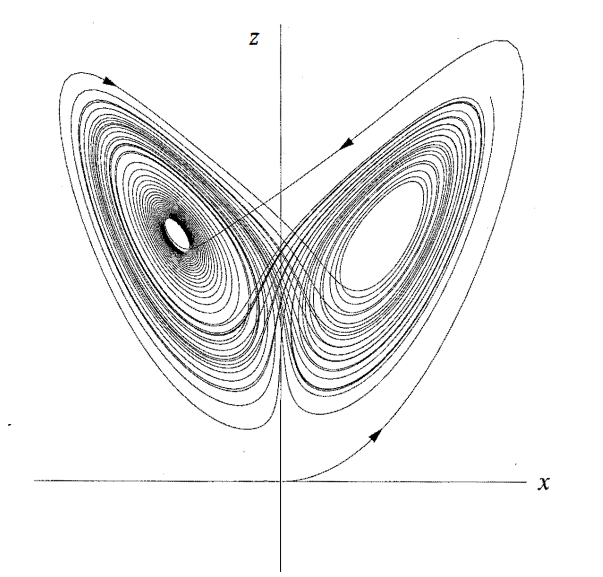
\includegraphics[width=0.6\textwidth]{fig/strange.png}
  \caption{Lorenz attractor. Image taken from Strogatz - Nonlinear dynamics and chaos}
  \label{figStrange}
\end{figure}
%
\subsubsection{Universality Of Complex Systems}
Not all complex systems are biological in nature.
In Dynamics of Complex Systems Yaneer Bar-Yam illustrates this as shown in fig
\ref{figCX}.
In the classical school of thought different fields are seen as divergent,
however Bar-Yam points out that each field deals with systems, and it turns out
that complex systems have much in common regardless of how and where they
originate.
This \emph{universality} is a powerful tool when studying systems such as neural
networks because it allows us to explain and study much of the behavior with far
simpler models, one such model being \emph{cellular automatons}.
\begin{figure}[h!]
  \centering
  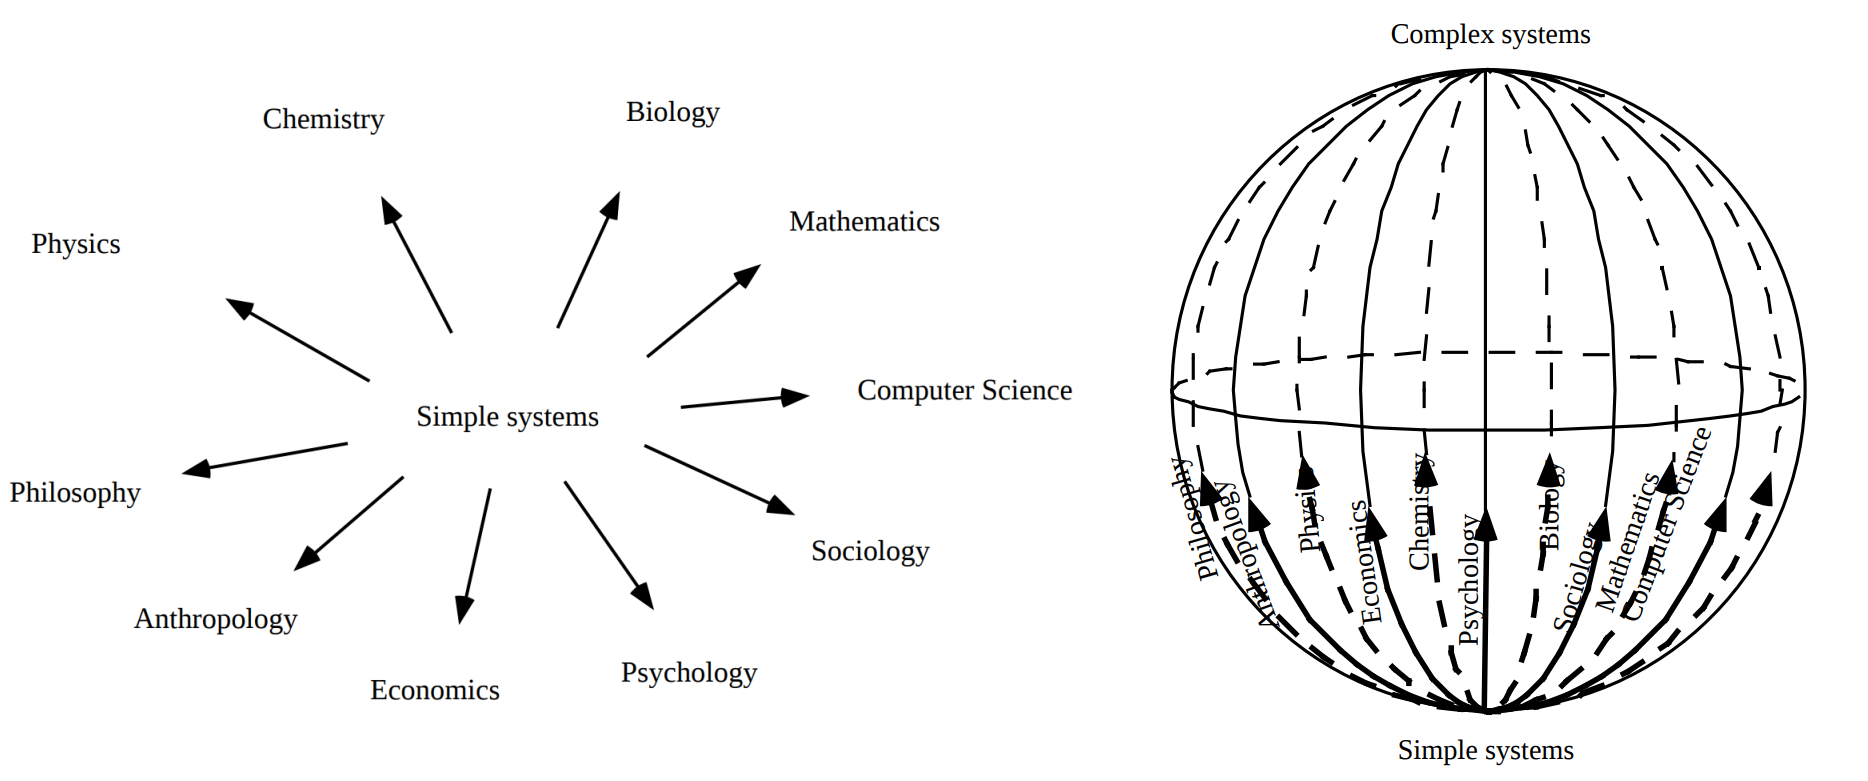
\includegraphics[width=1\textwidth]{fig/BarYamCX.png}
  \caption{
    Figure taken from Yaneer Bar-Yams Dynamics of Complex Systems showing how
    various fields converge towards complex systems rather than diverging.
  }
  \label{figCX}
\end{figure}
\subsection{Cellular Automata}
A \emph{Cellular Automaton}\footnote{Singular: Automaton, Plural: Automata}, CA
in short, is a simple discrete model of a single cell which changes between a
discrete set of states based only on its immediate neighbors.
Figure \ref{figCA22} shows an example of a \emph{rule set}, or \emph{transition
  table} for a cellular automaton with only two states, and an initial
configuration, or ``seed'', which over several steps forms a pattern.
%
CAs have many properties that make them ideal as a model for studying complex
systems and how they can facilitate computation.
The reasons for this can be seen in \ref{figSipperClass} from
\cite{sipper_emergence_1999}
showing how CAs model computation made by simple elements interacting locally in
a vastly parallel manner.
%
In other words, computation in CAs must be self organized, bottom up and driven by
local interaction which are the features that all complex systems share due to
universality.
%
An example of such a computation given by Sipper is contour extraction of an
image, highlighting how a parallel local computation can yield a global result.
%
While contour extraction is computation it is not very general, and the initial
conditions are set up in a rather artificial way, so one might ask if CAs can
perform more complex computation.
As it turns out the answer is yes, as even simple 1D CAs are \emph{Turing
  complete}, enabling them to express any computation.
This is of little practical use though, as Sipper puts it: ``This is perhaps the
quintessential example of a slow bullet train: embedding a sequential universal
Turing machine within the highly parallel cellular-automaton model'', however it
does show that more complex rules or models are not inherently more capable.
\begin{figure}[h!]
  \centering
  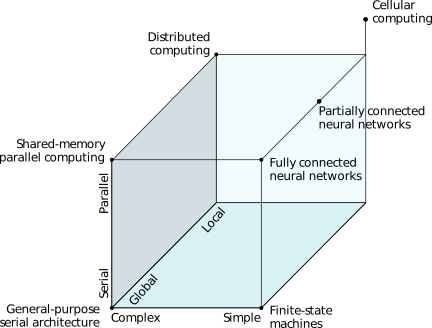
\includegraphics[width=0.6\textwidth]{fig/sipperComp.png}
  \caption{From Sipper paper.}
  \label{
    Figure taken from Sippers ermergence of cellular computation showing
    how computation can be separated by three orthogonal axes.
  }
\end{figure}
\begin{figure}[h!]
  \centering
  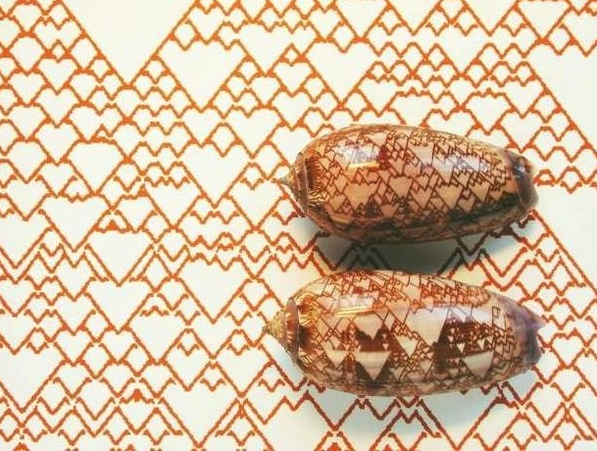
\includegraphics[width=0.6\textwidth]{fig/CApattern.png}
  \caption{
    The pattern on the shell is reminiscent of the background which is
    generated by a cellular automata, suggesting that CAs can model how nature
    generates patterns.
  }
  \label{figCX}
\end{figure}
\subsubsection{Order, Criticality and Chaos}
Contour extraction and turing machines are artificially constructed
computations, neither spontaneously occuring or particularily complex.
A pioneer in the field, Stephen Wolfram, was interested not only in expressing
computations with CAs, but in which conditions computation could spontaneously
occur.
He divided CAs into 4 classes based on their behavior, from least to most
complex, as shown in fig \ref{figPhase}.
Class 1 and 2 quickly resolved to static or simple periodic behavior, which
corresponds to an attractor landscape with many point and cyclic attractors with
shallow basins.
Class 3 CAs exhibited chaotic behavior where small differences in initial
conditions caused the systems to diverge quickly into cycles so long they could
effectively be considered to be in strange attractors.
Class was characterized by having very long transients, forming complex
patterns of localized structures corresponding to an attractor landscape with
fewer attractors with very large basins.
Wolfram correctly suspected that the fourth class was capable of computation,
even of the universal\footnote{Not to be confused with
  universality of complex systems} variety.
%
In Langton's pioneering paper \emph{Computation on the Edge of Chaos}
\cite{langton_computation_1990} Langton explores the space of possible
transition tables for one dimensional cellular automata, linking the space of CA
behavior to phase changes in material.
%
Langton ascribed a parameter, $\lambda$, to each ruleset which described how evenly
matched rules leading to the dead state was vs the live state.
When all configurations lead to one type of cell the ruleset $\lambda = 0$, while
the ruleset where the amount of states leading to dead and live are equal 
$\lambda = 1.0$
%
Langton found that the $\lambda$ parameter modeled how rulesets and wolframs CA
classes interact in a way analogous to how matter changes phase at different
temperatures, shown in \ref{figCAegg}.
%
Fig \ref{figPhase} is a phase diagram for water where the colored lines shows
first order phase changes, such as freezing below 0 degrees at ocean-level
pressure, analogous to how CAs go from fixed to periodic in \ref{figCAegg}.
%
More interesting, the figure also shows a \emph{critical point} where matter
undergoes a \emph{second order phase change} in which it exhibits properties of
several phases at once.
%
In the critical phase matter forms structures that are self-similar, a property
known as \emph{scale invariance}, which causes classical assumption about
``smoothness'' of behavior at lower scales that allows simplifying the lower
scale behavior break down.
%
This is a recurring theme for systems, at the \emph{edge of chaos} there is a
critical point where the forces of feedback and dampening are closely matched,
allowing a system to be responsive and dynamic without disintegrating into
chaos.
\begin{figure}[h!]
  \centering
  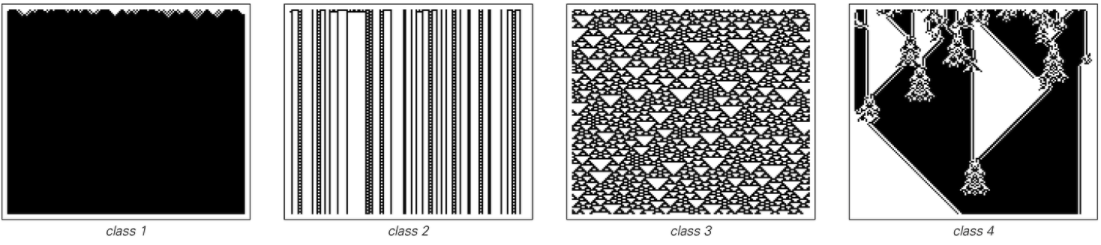
\includegraphics[width=1.0\textwidth]{fig/classesCA.png}
  \caption{Source: A new kind of science.}
  \label{figPhase}
\end{figure}
\begin{figure}[h!]
  \centering
  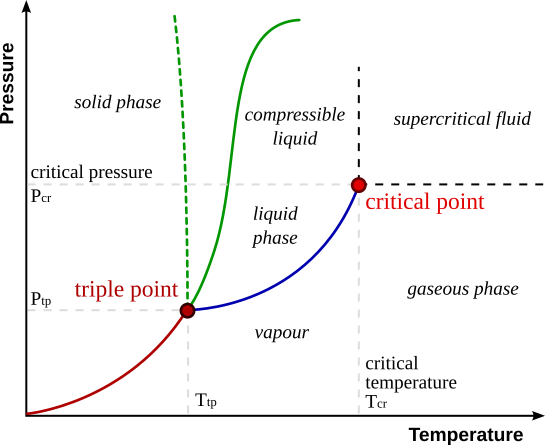
\includegraphics[width=0.5\textwidth]{fig/Phase.png}
  \caption{Source: wikimedia commons}
  \label{figPhase}
\end{figure}
\begin{figure}[h!]
  \centering
  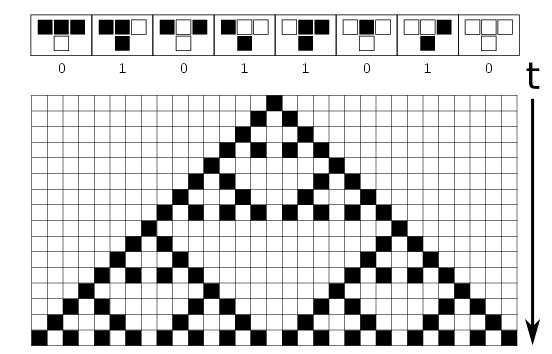
\includegraphics[width=1\textwidth]{fig/ca22t.png}
  \caption{
    The pattern generated from the rule 22 cellular automata with a
    single starting cell. The system is one-dimensional, but when rendering each
    step as the system evolves over time a two-dimensional image is created.
  }
  \label{figCA22}
\end{figure}
\begin{figure}[h!]
  \centering
  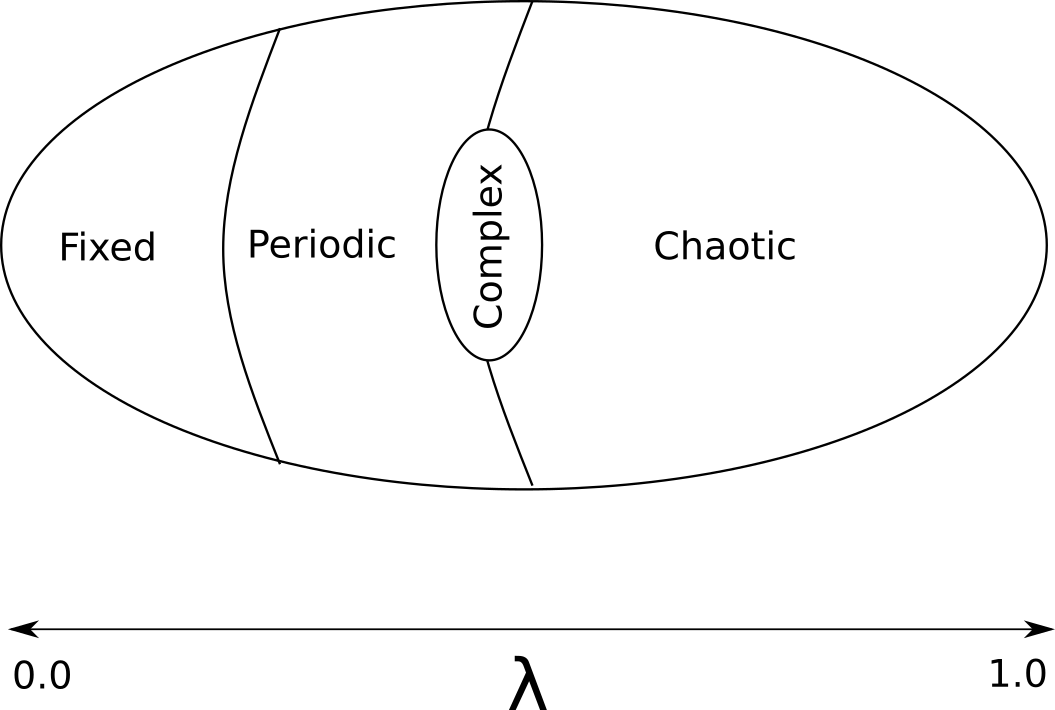
\includegraphics[width=1\textwidth]{fig/egg.png}
  \caption{Langtons egg, showing how a complex regime emerges at the edge of
    order and chaos}
  \label{figCAegg}
\end{figure}
\section{Material Computing}
Modeling neurons as cellular automata gives an idea of how neurons organize
themselves into computationally capable networks and how this computation may
look like, but the question of how to make sense of these dynamics and utilize
them.
Before tackling neurons it is necessary to extend our model to the physical
realm and develop a model that can be extended to perform computation.
A very natural extension of the CA model is \emph{material computing} in which
the atoms that make up matter locally interact in similar ways to CAs.
%
Two pioneers in this field were the british duo Pask and Beer which studied how
unstructured matter could be used to perform computational tasks.
%
In one experiment [cite ???] the duo used silver in an acidic solution which
would form short-lived silver filaments when subjected to electric currents.
%
By tuning the various knobs controlling parameters such as voltage this solution
could be made to perform the task of tone discrimination, proving that
unstructured matter could in fact perform computation.
%
In Langtons CAs the goal was not to compute, but to explore what conditions were
necessary for computation to occur, while Gordon and Pask sought to actually
compute by observing how the matter reacted to sound and tuning the parameters
in response.
%
Tommaso Toffoli argues that ``Nothing makes sense in computing except in the
light of evolution'' in his eponymous paper
\cite{tommaso_toffoli_nothing_nodate}, which separates Langtons compute capable
CAs and the tone discrimination which had been evolved by repeatedly observing
its performance and altering the parameters accordingly.
%
% TODO Hmm hmm hmm
A corollary of the turing completeness of cellular automatas is that CAs can be
``tuned'' in a rather heavy handed way to compute, but a more interesting
conjecture is that a CA with a random seed will eventually exhibit local
self-replicating behavior, spontaneously giving rise to what Toffoli would
regard as computation, or possibly even as life.\par
%
Whereas the pioneers in material computing sought to perform specific tasks with
their experiments more recent work has been made for general computation. One
approach is \emph{Evolution In Materio} (EiM) \cite{tufteEiMpaper} where various
materials have their parameters tuned algorithmically to perform a
transformation between input and output.
Figure \ref{figEiM} shows how the properties of a material can be tuned in
response to its performance on some task.
A recent effort, realizing the design in \ref{figEiM} is the NASCENCE project
which has developed a physical device, ``mecobo'' that can host a variety of
materials which can then be interacted with using an array of electrodes.
%
By using the same basic loop as the early material computing reasearchers the
Mecobo board has been used to create XOR logic gates using unstructured carbon
nano-tubes \cite{lykkebo_mecobo:_2014}.
%
% This gives latex error about missing dollarsign, but upon inserting text is no longer
% bold...
\begin{figure}[h]
  \centering
  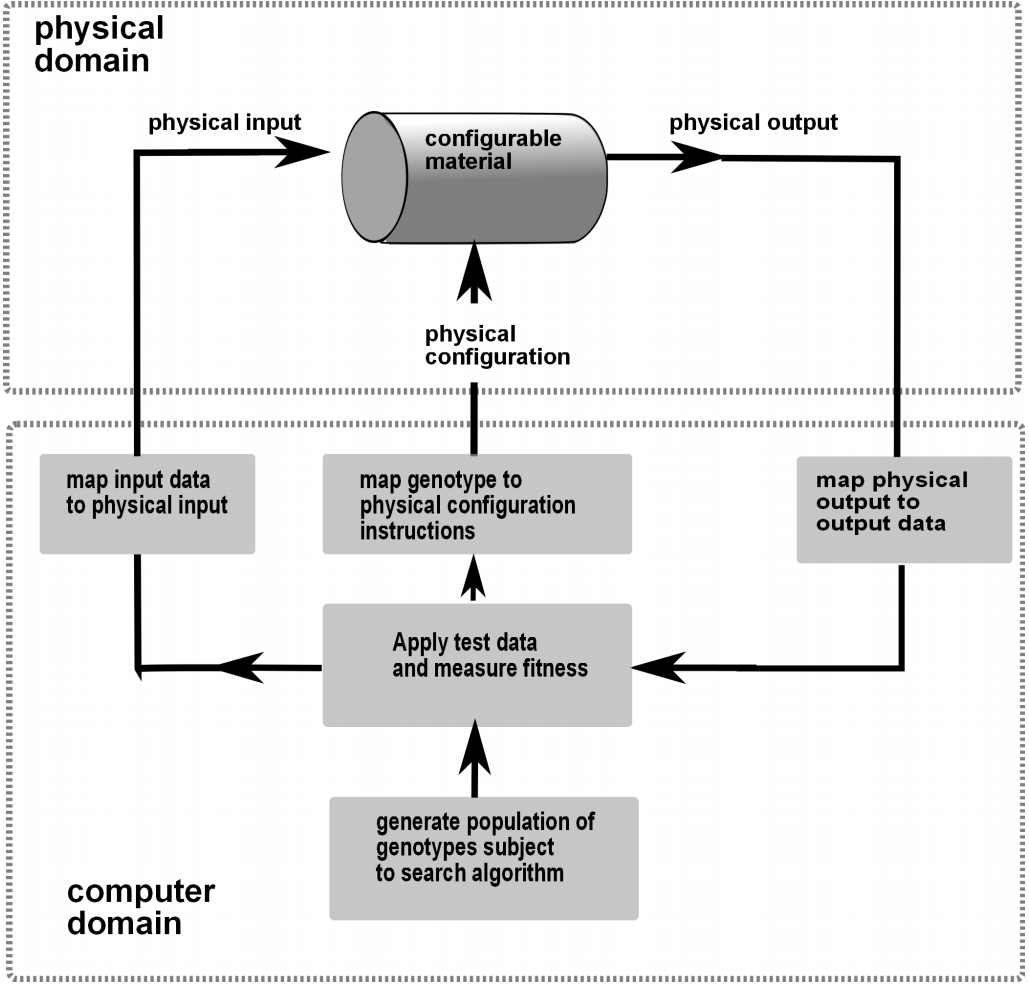
\includegraphics[width=1\textwidth]{fig/GunnarEiM.png}
  \caption{
    From \cite{tufteEiMpaper}, showing the framework of EiM using a genetic
    algorith.
  }
  \label{figEiM}
\end{figure}
\subsubsection{(DS)^2}
%
In the introduction Fernando's water bucket computer
\cite{fernando_pattern_2003} was briefly mentioned 
In their paper they refer to the bucket as a ``liquid brain''\footnote{Also in
  quotation marks in the original paper}, performing calculations by observing
the resulting wave pattern made by small motors.
Unlike its biological counterpart the ``liquid brain'' does not evolve over
time, in fact it has no structure to evolve at all, at least not at the chosen
scale of observation.
%
$(DS)^2$ is shorthand for dynamic systems with \emph{dynamical structure}, and
materials that exhibit this behavior can be used to study and model biological
systems.
In these material systems the \emph{state space}, that is the set of reachable
states, and the transition function between them evolve over time in tandem with
the systems dynamics, both shaping them and being shaped by them.
%
In \cite{eimDS2} Odd Rune shows that a mixture of table salt and
water exhibits (DS)2 behavior using the mecobo board by showing that the systems
response to perturbation evolves over time.
%
Simalirily, experiments using simulated artificial spin ice \cite{joh_ASI}
shows that in a lattice of nano-magnets several underlying microstates map to the
same macro-state as shown in fig \ref{figJohASI}.
This highlights the importance of observation level when describing systems.
One could choose to... Something something.
\begin{figure}[h]
  \centering
  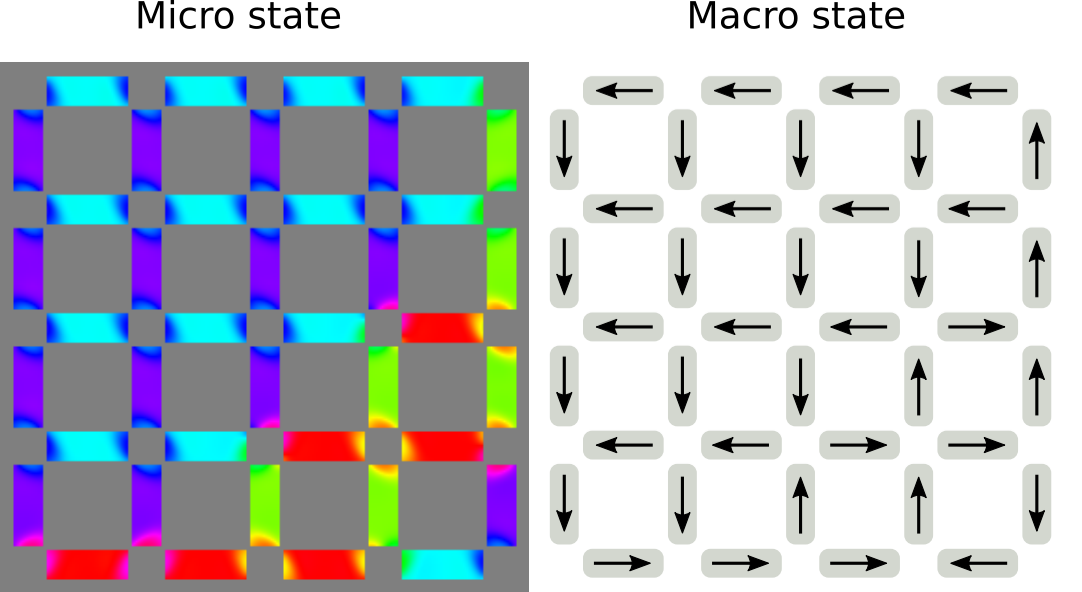
\includegraphics[width=1\textwidth]{fig/joh_ASI.png}
  \caption{
    A simulated lattice of nanomagnets from \cite{joh_ASI} allows us to peer
    into the micro state of a lattice of nanomagnets, with a corresponding macro
    state showing what would be measurable in a real system.
  }
  \label{figJohASI}
\end{figure}
\section{Computing Neural Networks}
Material computing provides both a theoretical framework and practical
approach for modeling and interacting with the computational capabilities of
living neural networks.
%
The $(DS)^2$ viewpoint is a very natural fit when modeling how neurons organize
into networks.
The structure in a neural network continously evolves as each neuron
individually seeks out other neurons to forge new connections while letting old
connections wither and die off.
The dynamics of a neural network is the electro-chemical communication between
neurons in the network.
These signals are obviously shaped by the topology of the neural network, but
they are also the driving force between the continued evolution of the networks
topology in ways that we only have a rudimentary understanding of.
%
Although both table salt and neural networks exhibit $(DS)^2$ behavior only the
neurons do this on purpose.
When viewing Pask's tone discrimination experient from a $(DS)^2$ viewpoint we
can catch a glimpse of the same process that shaped the rules governing neural
self organization.
Although this was not the view of the experimenter, the tuning of parameters
performed by Pask altered how silver filaments formed and decayed, which can be
viewed as a rudimentary approximation of how neurons form connections.
%
In Pask's experiment the observer tuning the knobs served the same role as
evolution did in shaping neurons, and neither force were particularily concerned
about exactly what the underlying structure of the material did as long as the
behavior of the material performed as desired on a macro-scale.
%
\subsubsection{The Computing Neuron}
The neuron, or nerve cell, is the basic building block of both the human brain
and the nerve system.
The culmination of billions of years of evolution, the neuron is a vastly
complex entity, featuring complex chemical pathways and gene regulatory
networks.
However, as discussed in the section on complexity, this behavior is nescessary
in order for evolution to function.
As a corollary, most of the complexity of the neuron is not nescessary for it to
function, it is simply a byproduct of evolution, an implementation detail.
It is the view of the author that the behavior of a neural network can be
modeled with a much simpler neuron such as in artificial spiking neural
networks.\par
Although the computation performed by neurons can be modeled with simpler
models, the fact of the matter is that the cyborg project utilizes real neurons
rather than a digital approximation, so a cursory introduction of the neuron is
in order.
While there exists a multitude of different neurons in the human body it is
sufficient to consider a simplified model neuron, shown in fig [a figure of a
neuron].
The three three main parts are the body, or \emph{Soma}, the \emph{Dendritic
  network} and the \emph{Axon}. 
The dendritic network acts as a receptor sensing electrical activity around the
neuron, while the axon transmits electric pulses to neighboring cells.
The connection between two neurons is called a \emph{Synapse}.
%
In addition to chemical signals neural networks communicate and regulate their
behavior through chemical signals.
These chemical signals, known as neurotransmitters, correlate strongly with
electrical activity however, thus measuring the chemical gradients in neural
networks is not a priority from a compuational perspective.
\subsubsection{Neural Dynamics}
The ``medium'' of communication between neurons chosen as the observable macro
state, that is the dynamics we are interested in measuring for the neural
network are electrical bursts of activity, known as spikes.
Figure \ref{figWave} shows recorded activity from an electrode.
Each electrode measures the activity of the surrounding neurons rather than the
state of a single neuron.
Given that spikes propogate through the network in a cascading manner this
level of observation is sufficient and more fine grained measurements is not a
priority.
Over time these dynamics evolve in tact with the structure of the network, as
expected in the section on $(DS)^2$.
Not only does the dynamics of the neural network change like the table salt
experiment, it moves in the complexity space as shown in \ref{figDopey} towards
a critical phase as discussed in the section on cellular automata.
%
\begin{figure}[h]
  \centering
  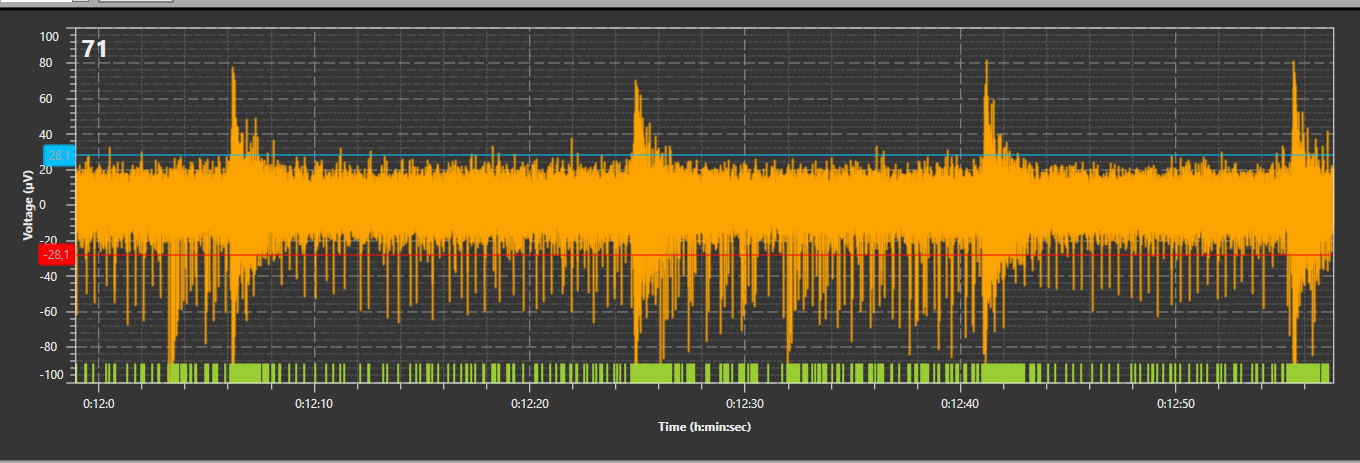
\includegraphics[width=1\textwidth]{fig/PacemakerBurst.png}
  \caption{
    Electrical activity from the neural tissue is recorded at a micro-volt
    scale.
    In the depicted recording there is constant spiking interspersed with large
    bursts of activity.
  }
  \label{figWave}
\end{figure}
\begin{figure}[h]
  \centering
  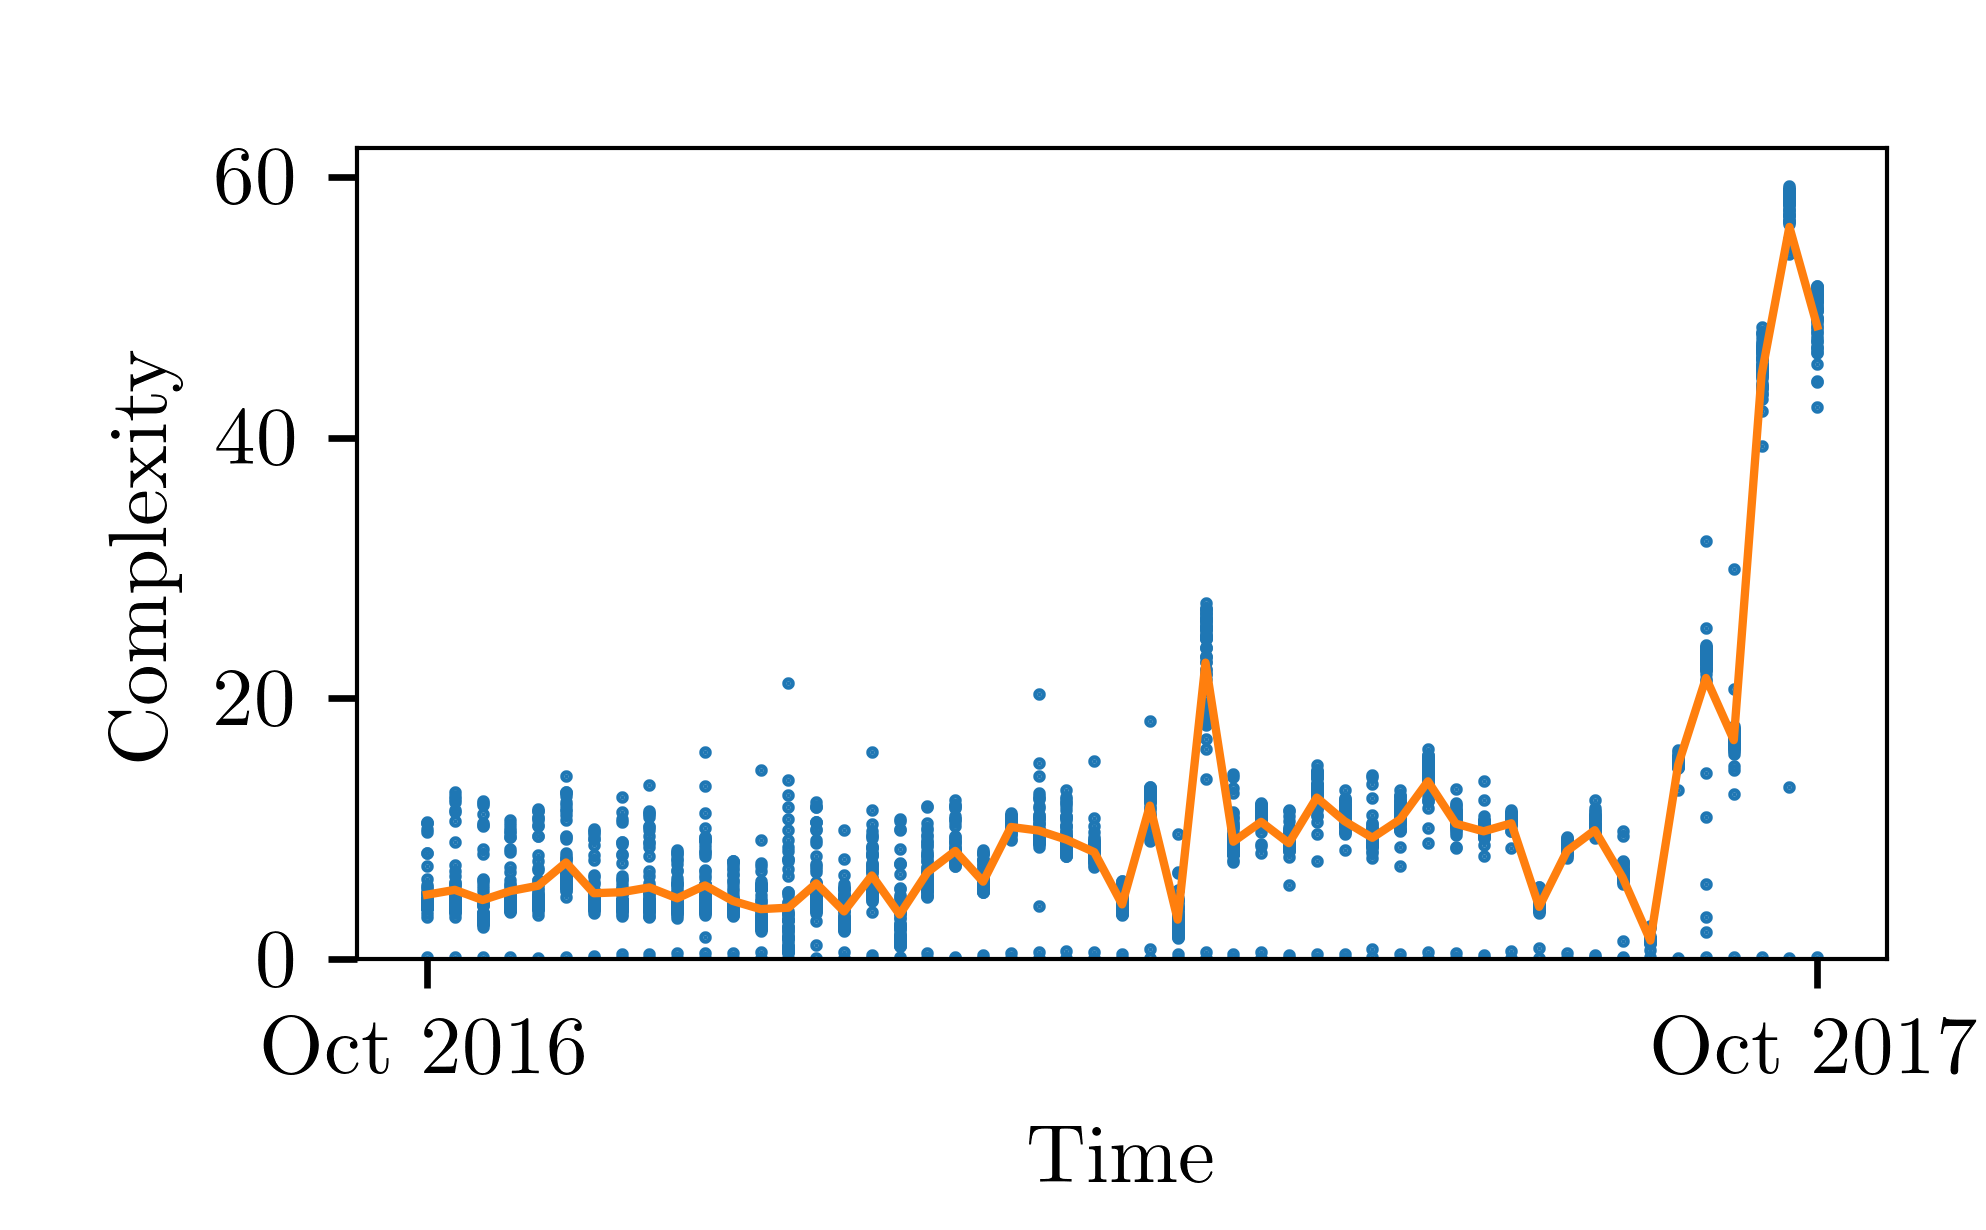
\includegraphics[width=1\textwidth]{fig/dopeyComplexity.png}
  \caption{
    Approximated Kolmogorov complexity of the firing patterns over a one year
    period.
  }
  \label{figDopey}
\end{figure}
\subsubsection{Artificial Neural Networks}
In recent years ANNs\footnote{Or rather, the advent of hardware capable of
  efficiently running and training them.} (shorthand for artificial neural
network) have revolutionized AI due to their ability to solve hard
classification problems such as image recognition.
The simplest, and most successful variation is the \emph{feed forward} topology
shown in \ref{figFFANN} in which each layer only interacts with the layer
directly in front and behind it.
Shown in \ref{figNeuronModel}, the model for a single neuron consists of a
summing function that calculates a weighted sum of incoming connections and a
function that calculates the outbound activation of that neuron.
More advanced models of neurons often retain state from their previous
activation, one such variant being the spiking neuron which emulates the
biological neuron more faithfully.
Networks with neurons that retain state can have more interesting topologies
where the connections between neurons can go in all directions.
Cleary recurrent spiking neural networks should be more capable than feed
forward networks, if nothing else for their ability to encode time-series as
part of their state, yet the simple, non-spiking variant has proven much more
successful.
This gap stems from the relative simplicity of the fitness landscape of simpler
network topologies which allows training algorithms to manually adjust the
weights between layers iteratively until a good result is achieved.
In back-coupled networks however the relation between cause and effect is far
more obscure, thus algorithms which essentially assign blame and alter weights
based on this are unable to cope with these topologies.
\begin{figure}[h!]
  \centering
  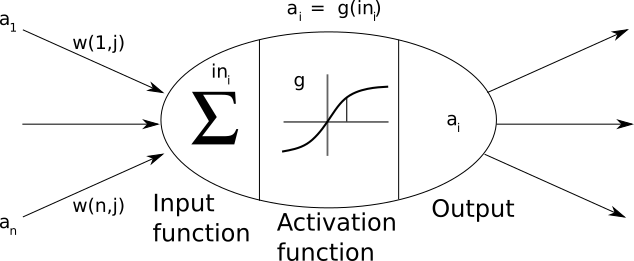
\includegraphics[width=0.7\textwidth]{fig/ArtificialNeuron.png}
  \caption{An artificial neuron}
  \label{figNeuronModel}
\end{figure}
\begin{figure}[h!]
  \centering
  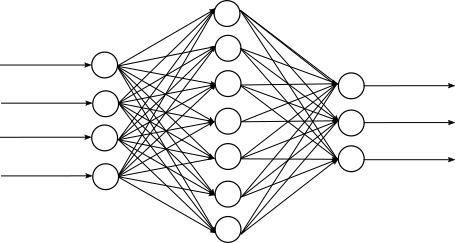
\includegraphics[width=0.7\textwidth]{fig/feedforward.png}
  \caption{A feed forward ANN.}
  \label{figFFANN}
\end{figure}
% Få inn RC fig tidligere
\section{Reservoir Computing}
Material computing has provided a tractable model of how the neuron computes and
how to physically interface with them.
However, still absent is a model that allows us to actually access the
computational capabilities.
In fact, from the field of material computing Susan Stepney extends the
following warning ``the biological substrate is extremely complex and
complicated, having evolved over billions of years to exploit specific
properties. In some sense, biological substrate is as far (or further!) removed
from a primitive substrate as are our own designed abstract digital
computational media.''
%
As the heading indicates, the ace up our sleeve comes in form of \emph{Reservoir
  Computing}, a technique that fittingly enough originated from the study of
ANNs of the back-coupled variety\cite{jaeger_echo}[Cite Maass].
In \cite{jaeger_echo} randomly connected neural networks are used to solve
classification problems, forgoing training the network altogether.
Instead the randomly generated network was used as a \emph{reservoir} of
dynamics that reacted to the input while a simple linear output function had to
be trained.
The principle behind reservoir computing is to employ a complex system as a
reservoir which, as Schrauwen puts it \cite{schrauwen_overview_2007} ``... acts
as a complex nonlinear dynamic filter that transforms the input signals using a
high-dimensional temporal map, not unlike the operation of an explicit, temporal
kernel function.''
Figure \ref{figRC} shows this setup, in which input perturbs a reservoir and the
resulting dynamics is classified using a linear filter.
%
In order to explain why this works, schrauwen makes a comparison to the the
machine learning technique of source vector machines work, as shown in fig
\ref{figSVM}.
The general idea behind an SVM is to expand the input into a higher dimensional
``feature space'', which in the figure is represented by the transition from 2D
to 3D.
% Altså sensitivitet til input conditions
Similarily, when perturbed by some initial condition the resulting dynamics from
the reservoir can be interpreted as a feature space and a trained \emph{readout
layer} can interpret the resulting dynamics.
Schrauwen points out two major differences between SVMs and RCs.
First, SVMs only implicitly expands the input to high dimensional space in order
to make the problem tractable, while reservoirs do not.
Secondly, kernels are not capable of handling temporal signals.
% %
The second difference is very important, it is what allows reservoirs to
implicitly encode temporal signals in their dynamics, making reservoirs a
natural fit for tasks such as speech recognition where each part of the input is
context sensitive.
\begin{figure}[h!]
  \centering
  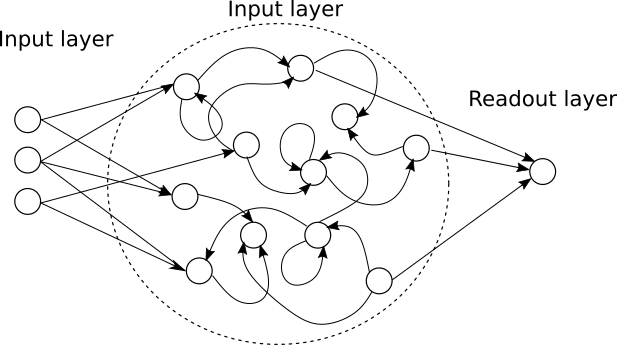
\includegraphics[width=0.7\textwidth]{fig/reservoirz.png}
  \caption{
    A generic reservoir computer setup. Inputs are fed into the reservoir as
    perturbations, and the resulting dynamics are classified by a readout layer.
  }
  \label{figRC}
\end{figure}
\begin{figure}[h!]
  \centering
  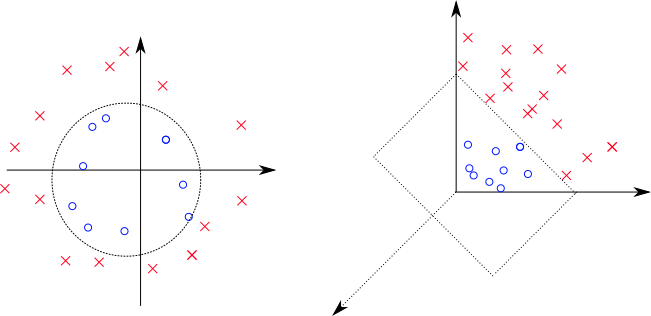
\includegraphics[width=0.6\textwidth]{fig/svmthing.png}
  \caption{
    With the SVM approach the input is processed by a kernel function that
    creates a high dimensional feature space that is linearily separable.
  }
  \label{figSVM}
\end{figure}
\subsection{Linear and nonlinear output layers}
In classical reservoir computing emphasis is put on the readout layer being
linear.
This is important because when solving a classification problem as the one in
\ref{figSVM} a linear classifier ensures that the actual problem-solving happens
in the reservoir rather than the output layer.
When using an artificial neural network as readout layer with more than a single
layer (known as a perceptron) the layer can, given enough nodes approximate any
nonlinear function.
This is a reasonable constraint when proving that nonlinear computation is done
by the reservoir, but the case for removing this constraint can be made.
A simple case can be made showing a reservoir with a nonlinear output layer can
achieve a better performance on a classification problem.
Another case is made for problems with a temporal aspect where the readout layer
has only a limited memory.
In this case simply showing that the problem can be solved is not sufficient,
the reservoir could be a simple memory bank doing no nonlinear classification
itself, thus it is still necessary to show a performance increase over
traditional methods.
It is not clear whether there is any advantage to using a nonlinear filter for
neural cultures, but for a proof of concept both approaches can be employed,
keeping in mind the caveats of using a nonlinear filter.
\cleardoublepage

%%% Local Variables:
%%% mode: latex
%%% TeX-master: "../main"
%%% End: